\chapter{State of the Art}
\chaptermark{State of the Art}
\label{chapter:soa}
\minitoc

%%%%%%%%%%%%%%%%%%%%%%%%%%%%%%%%%%%%%%%%%%%%%%%%%%%%%%%%%%%%%%%%%%%%%%%%%%%%%%%%%%%%%%%%%%%%%%%
\section{Introduction}
This chapter provides an overview of related work to contextualize the primary objectives of this thesis. Firstly, in Section~\ref{section:ift}, Information Flow Tracking (IFT) is introduced, detailing the different types and their respective purposes. We will discuss the various levels of monitoring, from program behaviour to the detection of hardware trojans.
Then in Section~\ref{section:physicalAttacks}, Physical Attacks are examined, focusing on two main types: Side-Channel Attacks (SCA) and Fault Injection Attacks (FIA).
Finally in Section~\ref{section:countermeasuresAgainstFIA}, as this work will concentrate on FIA, we will exclusively present countermeasures against Fault Injection Attacks.

%%%%%%%%%%%%%%%%%%%%%%%%%%%%%%%%%%%%%%%%%%%%%%%%%%%%%%%%%%%%%%%%%%%%%%%%%%%%%%%%%%%%%%%%%%%%%%%
\section{Information Flow Tracking}
\label{section:ift}
The concept of \textit{Information Flow Tracking} has been introduced by the work of Bell and LaPadula~\cite{BLP-76-military} and by Denning~\cite{D-76-commacm} in 1976.
This section introduces Information Flow Tracking mechanisms, explains how they work, and presents the various types of IFT with their different functional levels.
    
%%%%%%%%%%%%%%%%%%%%%%%%%%%%%%%%
\subsection{Different types of IFT}
There are two distinct types of IFT approaches: static and dynamic, each with its own specific objectives.

\subsubsection{Static IFT}
Static Information Flow Tracking (SIFT) is a security technique used to analyse and control the flow of information within a program or system without executing it, by examining the source code or compiled binary~\cite{HAK-21-acmcsur}. This method is particularly useful for identifying theoretical vulnerabilities, ensuring compliance with design principles, and preventing unauthorised information leaks before deployment. SIFT is comprehensive, covering all possible execution paths and detecting both explicit information flows (direct data assignments) and implicit flows (leaks through control flow structures). By performing checks at compile-time, SIFT helps developers address potential security issues early, enforcing principles like non-interference and data confidentiality through security policies. However, static analysis may generate false positives by flagging theoretical flows that might not occur in practice and may struggle with certain dynamic language features or runtime-dependent behaviours. SIFT is employed in various contexts, such as verifying secure information flow in operating systems, programming languages with built-in information flow controls, and hardware design for secure systems.

\subsubsection{Dynamic IFT}
Dynamic Information Flow Tracking (DIFT) is a powerful security technique that monitors and analyses, in real-time, the flow of information within a program during its execution~\cite{CGDJ-21-micromac}. DIFT operates by tagging or labelling input data from potentially untrusted sources and tracking how this data propagates through the system~\cite{SLD-04-sigplan}. As the program executes, DIFT maintains metadata about the tagged information, updating it as operations are performed on the data. This allows the system to detect when tainted data is used in security-critical operations, such as modifying control flow or accessing sensitive resources. DIFT can be implemented at various levels, including hardware, software, or a combination of both. Hardware-based implementations often offer better performance but require specialized processor modifications, while software-based approaches provide more flexibility but may incur higher overhead~\cite{CGDJ-21-micromac}. DIFT has proven effective in detecting and preventing a wide range of security vulnerabilities, including buffer overflows, format string attacks, and code injection attacks~\cite{SLD-04-sigplan}. However, DIFT also faces challenges, such as handling implicit information flows, managing performance overhead, and addressing over-tainting issues.
This approach might not cover all potential data paths, as it is dependent on the specific conditions and inputs provided during the monitoring period.
Despite these challenges, DIFT remains a valuable tool for software security, particularly for runtime attack detection in modern systems.

%%%%%%%%%%%%%%%%%%%%%%%%%%%%%%%%    
\subsection{Different levels of DIFT}
IFT can be implemented at various levels of abstraction in computing systems~\cite{HAK-21-acmcsur, BSMCVEJCO-21-acmcsur,CGDJ-21-micromac}. Each level presents unique trade-offs between precision, performance overhead, and ease of implementation, allowing designers to choose the most appropriate approach for their security requirements.

Software-based DIFT mechanisms benefit from close integration with the software context via binary code instrumentation and source code modifications, offering better flexibility, customisation, and scalability without altering hardware components. However, these software solutions often incur high performance overheads due to the extra instructions required. They operate at either the system level, monitoring OS-wide information flows, or the program level, focusing on specific applications.
On the other hand, hardware-assisted DIFT designs can efficiently enforce security rules by implementing DIFT-related operations as hardware logic, reducing performance overhead but at the expense of flexibility and scalability, making them challenging to deploy in modern commercial systems. They can be implemented within processor cores or as off-core designs. But they can also be at the lowest level, such as Gate-Level IFT who tracks information flow through logic gates.
A hybrid hardware and software co-design offers a promising alternative, enabling fine-grained security checks by associating software context with hardware data, though it faces challenges such as balancing flexibility with hardware overhead and designing appropriate tags that support rule updates post-deployment.

Figure~\ref{fig:levels_system} represents the different levels of a simplified embedded system: application layer, system service layer, OS layer, and hardware layer. This figure is inspired by Figure 1.9 of~\cite{ebrary}. Software-based IFTs work in the first three levels.

Positioned at the highest level of the software hierarchy, \textit{the application layer} is responsible for implementing system functionalities and business logic. Functionally, all modules within this layer work together to execute the required system operations. Applications generally run in a less-privileged mode on the processor and utilise the OS-provided API scheduling to communicate with the operating system.
\textit{The system service layer} serves as the intermediary service interface offered by the OS to the application layer. This interface allows applications to access a variety of OS-provided services, essentially bridging the gap between the OS and applications. Typically, this layer encompasses components like the file system, Graphical User Interface (GUI), task manager.
An Operating System (OS) is a software framework designed to manage hardware resources uniformly. It abstracts numerous hardware functions and offers them to applications as services. Common services provided by an OS include scheduling, file synchronisation, and networking. Operating systems are prevalent in both desktop and embedded systems. In the context of embedded systems, OSs possess distinct characteristics such as stability, customisability, modularity, and real-time processing capabilities.
\textit{The hardware layer} refers to the physical components and circuitry, including the microprocessor or microcontroller, memory, sensors, and input/output interfaces. This layer encompasses all the tangible electronic elements that interact directly with each other to perform the device's functions. It provides the essential infrastructure that supports and drives the embedded system’s operations and connectivity.

\begin{figure}[ht]
    \centering
    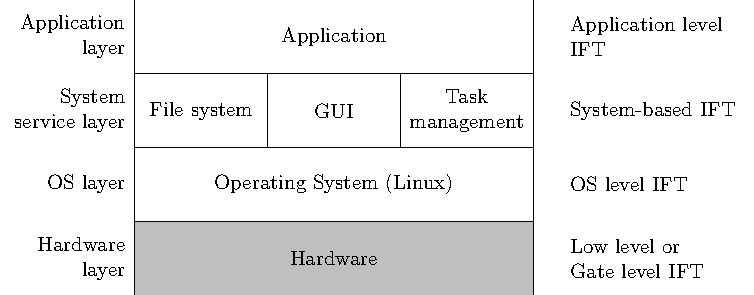
\includegraphics{c2_soa/img/system_layer.pdf}
    \caption{Simplified representation of the different layers in an embedded system}
    \label{fig:levels_system}
\end{figure}

Tracking information can be performed at various levels, from the application level to the hardware level. Each level offers distinct advantages and disadvantages.
For instance, application-level tracking might provide detailed insights and user-friendly interfaces, while hardware-level tracking offers more granular data and real-time monitoring but can be more complex and costly.
The following subsections will explore these different levels, highlighting their respective benefits and limitations.


\subsubsection{Software-based DIFT}
\paragraph{Application level DIFT} tracks information flows between application variables. The programmer has to integrate data tagging inside his program and use a modified compiler or analyse his program to check if no security violation happened.
One application for DIFT at application level is language-based. Several security extensions have been proposed for existing programming languages.
JFlow~\cite{M-99-popl} is one of the first works that has described an extension of the Java language by adding statically-checked information flow annotations.

Multiples works introduce DIFT extensions for different languages, for example, such as JavaScript~\cite{CN-15-ccs, AF-09-plas}.
Austin et al.~\cite{AF-09-plas} propose a method for tracking information flow in dynamically-typed languages, focusing on addressing issues with implicit paths through a dynamic check. This approach avoids the necessity for approximate static analyses while still ensuring non-interference. The method employs sparse information labelling, keeping flow labels implicit where possible and introducing explicit labels only for values crossing security domains.

Kemerlis et al.~\cite{KPJK-12-sigplan} provide a framework, \textit{libdft}, which is fast and reusable and applicable to software and hardware. \textit{libdft} provides an API for building DFT-enabled tools that work on unmodified binaries.

\paragraph{OS level and System-based DIFT} track and tag files (read or written) used by the application.
The main advantage of this approach is that it reduces the number of information flows, which lead to an improvement of the runtime overhead. In the other side, the main disadvantage of this approach is that it results in more false positives than the application-level approach.

TaintDroid~\cite{EGHTCCJMS-14-tocs} introduces an extension to the Android mobile phone platform designed to monitor the flow of privacy-sensitive data through third-party applications. Operating under the assumption that downloaded third-party applications are untrusted, TaintDroid tracks in real-time how these applications access and handle users’ personal information. The primary objectives are to detect when sensitive data is transmitted out of the system by untrusted applications, and to enable phone users or external security services to analyse these applications. They store the data adjacent to data for spatial locality. This may cause large performance and storage overheads, as the tag fetching requires extra clock cycles for memory access.
HiStar~\cite{ZBKM-11-commacm} is a new OS that has been designed to provide precise data specific security policies. The authors made the choice to assign tags to different objects in the operating system instead of data.


\subsubsection{Software and Hardware Co-Design-Based DIFT}
This type of design combines the features of both software DIFT and hardware DIFT. Using binary instrumentations and a modified compiler, the hardware and software co-design can provide the best of these two categories of DIFT: flexible security configuration and fine-grained protection with low impact on performances~\cite{CGDJ-21-micromac, BSMCVEJCO-21-acmcsur}.

One example of this type of DIFT is RIFLE~\cite{VBCROBRVA-04-micro}, a runtime information-flow security system designed from the user's perspective, provides a practical means to enforce information-flow security policies on all programs by leveraging architectural support.
RIFLE employs binary instrumentation and architectural support to enforce information flow security policies during runtime. The conventional Instruction Set Architecture (ISA) is transformed into an Information-Flow Security (IFS) ISA using a dedicated binary translator. Each instruction in the ISA corresponds to an instruction in the IFS ISA. 
In the IFS ISA, additional security registers are assigned to hold tags. To avoid the pitfalls dynamic mechanisms encountered while tracking implicit flows, the binary translation will convert all implicit flows to explicit flows. The RIFLE architecture is then responsible only for tracking explicit flows. The translated binary is executed within a modified processor supporting the IFS ISA, which is simulated within the Liberty Simulation Environment. RIFLE works with every programs that run on a system, and policy decisions are left to the user, not the programmer.

Townley et al.~\cite{TKPAY-19-micro} presented LATCH, a generalizable architecture for optimizing DIFT. 
LATCH exploits the observation that information flows under DIFT exhibit strong spatial and temporal locality, with typical applications manipulating sensitive data during limited phases of computation. The main objective is to detect attacks on the integrity of the system. The architecture consists of a software-assisted hardware accelerator (S-LATCH) running on a single simulated core. The software component of S-LATCH propagates tags, while the hardware accelerator monitors the data accessed by the program to detect tags. 

Porquet et al.~\cite{PS-13-codes} presented WHISK, a whole system DIFT architecture implemented within a hardware simulator. WHISK stores tags and data separately in memory locations to keep low area overhead and improve flexibility and to better accommodate the integration of hardware accelerators.. Tag insertion, storage, and access to the custom hardware are delegated. The software subsystem uses MutekH exokernel-based OS and provides support for tag page allocation, page table cache configuration, and interrupt handling concerning writes to untagged pages.


\subsubsection{Hardware-based DIFT}
Dalton et al.~\cite{DKK-07-sigarch} report that software DIFT solutions add significative runtime overhead, up to a slow-down of 37 times ! Therefore, in order to improve the execution time to be more on-the-fly, the idea is to directly implement the DIFT into the hardware, but the trade-off is flexibility.
This subsection discusses the hardware-based DIFT designs, including gate-level DIFT designs and micro-architecture-level DIFT designs. Surveys~\cite{HAK-21-acmcsur,BSMCVEJCO-21-acmcsur} present an overview on all hardware DIFT techniques. They developed a taxonomy for them and use it to classify and differentiate hardware DIFT tools and techniques.

\paragraph{Gate-Level DIFT} include gate-level netlist and also RTL designs. The goal is to protect against hardware trojans and unauthorized behaviours. To achieve that, during the creation of the circuit, additional logic is added for each gate used in the design.

GLIFT~\cite{TWMMCS-09-asplos} is a well-established IFT technique. The goal is to protect against hardware trojans and unauthorized behaviours. All information flows, both explicit and implicit, are unified at the gate level. GLIFT employs a detailed initialisation and propagation policy to precisely track each bit of information flow, by adding additional logic for each gate used in the design. By analysing how inputs influence outputs, GLIFT accurately measures true information flows and substantially reduces the false positives typically associated with conservative IFT techniques.
Hu et al.~\cite{HOITSMK-11-tcad} established the theoretical foundation for GLIFT. They introduced several algorithms for generating GLIFT logic in large digital circuits. Additionally, the authors identified the primary source of precision discrepancies in GLIFT logic produced by various methods as static logic hazards or variable correlation due to reconvergent fanouts. Many other works have been done on GLIFT to attempt a decrease of the logic complexity.

\paragraph{Off-Core DIFT} operations are performed on a dedicated coprocessor working in parallel of the main core.
The main drawback is that this approach needs a support from the OS for the synchronisation between data computations and tags computations in order to stall one core if it needs to wait the other. But on the other hand, its advantage is that it does not require internal hardware modifications to the main kernel. Processor manufacturers do not prioritise this type of security, and as most processors are not open to the public, it is difficult to modify them.

Kannan et al.~\cite{KDK-09-dsn} described one of the first work using a coprocessor to improve tag computation runtime overhead. Traditional hardware DIFT systems require significant modifications to the processor pipeline, which increases complexity and design time. Figure~\ref{fig:offcore_dift} represent how an off-core DIFT would be implemented. Kannan et al. uses this idea for implementing their solution of DIFT.
This coprocessor handles all DIFT functionalities, synchronizing with the main processor only during system calls. This design eliminates the need for changes to the processor's pipeline, logic, or caches, making it more attractive. The coprocessor is small, with an area footprint of about 8\% of a simple RISC core, and introduces less than 1\% runtime overhead for SPECint2000 applications benchmark. The paper demonstrates that the coprocessor provides the same security guarantees as integrated DIFT architectures, supporting multiple security policies and protecting various memory regions and binary types. This approach offers a balanced solution in terms of performance, cost, complexity, and practicality compared to existing DIFT implementations.

\begin{figure}[ht]
    \centering
    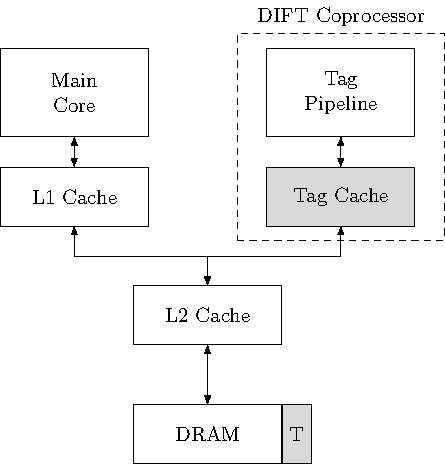
\includegraphics{c2_soa/img/offcore.pdf}
    \caption{Representation of a Hardware Off-Core DIFT (inspired by Figure 1 of~\cite{KDK-09-dsn})}
    \label{fig:offcore_dift}
\end{figure}

Wahab et al.~\cite{WCAHBLG-18-reconfig,WCAHLG-17-fpl} developed a DIFT using the ARM CoreSight debug component to extract a trace.
However, the debug component could only extract limited information about the application executing on the core. Therefore, some instrumentations have been required to recover the complete program trace. The information obtained from the trace is then sent to a dedicated DIFT coprocessor, which analyses the instruction trace and propagates tags according to a security policy. In terms of performance and area footprint, \cite{WCAHLG-17-fpl} gives around 5\% communication overhead and an area overhead of 0.47\% and a power consumption increased by 16\%; while~\cite{WCAHBLG-18-reconfig} gives a communication overhead of 335\%, an area increased by 0.95\% and a power consumption increased by 16.2\%. These results can not be compared to the initial design, as they use a coprocessor without the ARM core results.

\paragraph{Off-Loading DIFT} use a dedicated core of a multicore CPU~\cite{CKSFGMRRRV-08-sigarch,VHYR-08-cca,RGMRCKR-08-spaa}. Figure~\ref{fig:offloading_dift} represents how Off-Loading DIFT works with a core running the application and another, in parallel, run the DIFT analysis on the application trace. The application core is modified to create a trace and compress it. The trace includes executed instructions and packs main information such as PC address, register operands. This trace is then sent to the DIFT core via the L2 cache. Finally, the security core will decompress the trace and realizes tag computation in order to check whether an illegal information flow has been done. The notion of illegal information flow is specified thanks to a DIFT security policy.
The main advantage is that hardware does not need to know DIFT tags or policies and does not need a coprocessor with the management of the synchronisation between the two processors.  But the main drawback is that it requires a multicore CPU but reduces the number of core available and doubles the energy consumption due to the application trace analysis. In an embedded system where consumption is a critical factor, this solution is difficult to consider.

\begin{figure}[ht]
    \centering
    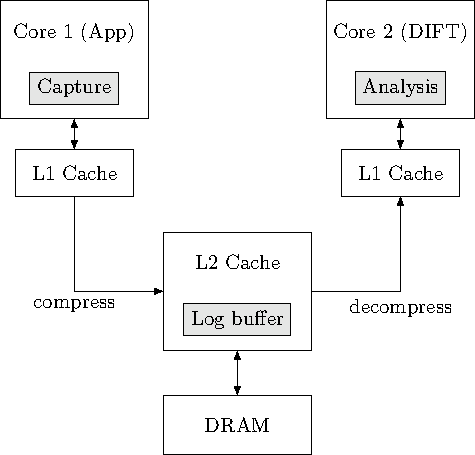
\includegraphics{c2_soa/img/offloading.pdf}
    \caption{Representation of a Hardware Off-Loading DIFT (inspired by Figure 1 of~\cite{KDK-09-dsn})}
    \label{fig:offloading_dift}
\end{figure}

\paragraph{In-Core DIFT} rely on a deeply modified processor pipeline which need to integrate tag computations inside the main core in parallel of data computations. This approach is highly invasive, but does not require any additional cores or coprocessors to operate and introduces no overhead for intercore synchronisation. Overall, its performance impact in terms of clock cycles over native execution is minimal. On the other hand, the integrated approach requires significant modifications to the processor core. All pipeline stages must be modified to add tags, a dedicated register file and first level of caches must be added to store tags in parallel with the regular blocks into the processor core. Figure~\ref{fig:incore_dift} shows the architecture of an In-Core hardware DIFT. When the processor fetches an instruction, its associated tag is sent in parallel. In the decode stage, the instruction is decoded while the security decode module decode the security policy to determine how the tag should be propagated and checked. When the instruction is executed, the tag is sent to a tag ALU to be checked. Then, if the tag is conforming to the security policy, the tag and the ALU output will be saved into the Data-Cache to be used again or stored in memory. Otherwise, if the tag is not conforming, the DIFT mechanism will detect the security violation and can raise an exception, stop the application, depending on what is configured.

\begin{figure}[ht]
    \centering
    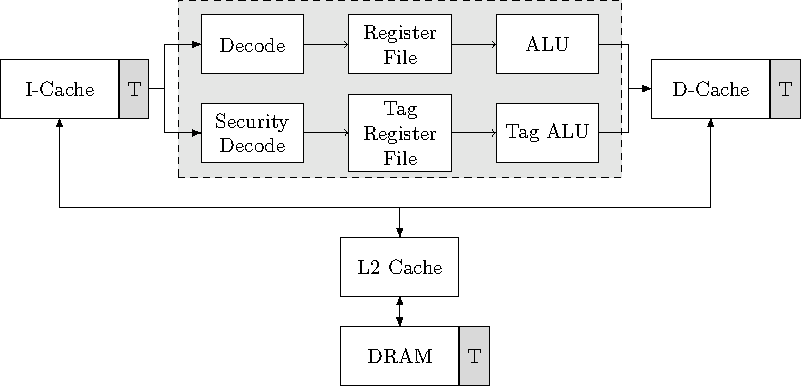
\includegraphics{c2_soa/img/incore.pdf}
    \caption{Representation of a Hardware In-Core DIFT (inspired by Figure 1 of~\cite{KDK-09-dsn})}
    \label{fig:incore_dift}
\end{figure}

Suh et al.~\cite{SLD-04-sigplan} proposed an approach in which the OS identifies a set of input channels as spurious, and the processor tracks all information flows from these inputs. Thanks to this tracking, the processor can detect various attacks such as attack targetting instructions or jump addresses. If the security policy detects something malicious in hardware, the OS will process the exception. They use 1-bit tag which means only two ways of representing security levels. They present two security policies that track differing sets of dependencies. Implementing the first policy incurs, on average, a memory overhead of 0.26\% and a performance decrease of 0.02\%. The second policy incurs, on average, a memory overhead of 4.48\% and a performance decrease of 0.8\%, and requires binary annotation unlike the first policy.

Dalton et al.\cite{DKK-07-sigarch} presented a DIFT architecture, Raksha, to support a flexible security configuration at runtime. They extended all storage locations including registers, caches and main memory with tags, they modified the ISA instruction to propagate and check tags. In this solution, they use 4-bits tags for each word. These tags represent the security policy and not the data state (e.g. trusted or untrusted). The authors provided two global sets of configuration registers, i.e., Tag Propagation Registers (TPR) and Tag Check Registers (TCR), to configure the security policy at runtime. There is one pair of TPR/TCR for each of the four security policies. The configuration register could be configured only in trusted mode. Moreover, the tag propagation and check could only be disabled in trusted mode. However, the security policy is difficult to update when the architecture is deployed.
The Raksha prototype is based on the Leon SPARC V8 processor, a 32-bit open-source synthesizable core, and they mapped the design onto a FPGA board.

Palmiero et al.~\cite{PDGLC-18-hpec} implemented a DIFT framework, D-RI5CY, on a RISC-V processor and synthesized it on a Field Programmable Gate Array (FPGA) board with a focus on IoT applications. The proposed design tags every word in data memory with a 4-bits tag and every general register with a 1-bit tag. Similarly to~\cite{DKK-07-sigarch}, Palmiero et al.~\cite{PDGLC-18-hpec} also adopted global configuration registers to customise the rule of tag propagation and checking. Each type of instruction has its own rule and can be modified separately. This method provides a more fine-grain tracking than Raksha but lacks flexibility for security policy reconfiguration for different program contexts.


%%%%%%%%%%%%%%%%%%%%%%%%%%%%%%%%
\subsection{How DIFT works}
\wip{expliquer DIFT ici ? en détail avec les schémas explicatifs}

%%%%%%%%%%%%%%%%%%%%%%%%%%%%%%%%%%%%%%%%%%%%%%%%%%%%%%%%%%%%%%%%%%%%%%%%%%%%%%%%%%%%%%%%%%%%%%%
\section{Physical Attacks}
\label{section:physicalAttacks}

\subsection{Side-Channel Attacks}
\subsection{Fault Injection Attacks}
\cite{BCNTW-06-procieee}

% A fault is the cause of an error, that is, an incorrect program or circuit state. If the error caused by the fault does not propagate and the application execution ends normally, the fault is ineffective. On the contrary, the fault is effective if the error affects the application’s execution, causing a failure, an observed behavior different from that expected.
% In the context of electronic circuits, a fault refers to an unintended deviation from the normal operation of the circuit. Faults can occur due to various reasons such as manufacturing defects, environmental factors, ageing, or external interference. These faults can affect the performance, functionality, and reliability of the circuit.

% In fault injection, which is a testing method used to evaluate the robustness and reliability of electronic circuits, a fault is deliberately introduced into the system to observe its behaviour and identify potential vulnerabilities.

%%%%%%%%%%%%%%%%%%%%%%%%%%%%%%%%%%%%%%%%%%%%%%%%%%%%%%%%%%%%%%%%%%%%%%%%%%%%%%%%%%%%%%%%%%%%%%%
\section{Countermeasures against FIA}
\label{section:countermeasuresAgainstFIA}

%%%%%%%%%%%%%%%%%%%%%%%%%%%%%%%%%%%%%%%%%%%%%%%%%%%%%%%%%%%%%%%%%%%%%%%%%%%%%%%%%%%%%%%%%%%%%%%